\documentclass[8pt,oneside]{book}
\usepackage{zxjatype}
\setjamainfont[BoldFont=IPAゴシック]{IPA明朝}
\setjasansfont{IPAゴシック}
\setjamonofont{IPAゴシック}

% New line height: 1.05 * 1.2 = 1.26
\renewcommand{\baselinestretch}{1.05}

\usepackage{polyglossia}

% To be able to use '\-/' in place of '-' inside \code{}
% so that long function names containing hyphens 
% can be broken up after the hyphen:
\usepackage[shortcuts]{extdash} 

% So that file names with multiple dots don't confuse 
% graphicx package when using \includegraphics command:
\usepackage[multidot]{grffile}
\usepackage{graphicx}

\usepackage[usenames,dvipsnames,x11names]{xcolor}
\usepackage{amsmath}

% To use Libertine letters and numbers,
% but tx-style operators in math environment:
\usepackage[libertine]{newtxmath} 

% Workaround to fix mismatched left and right math delimiters. Taken from: 
% http://tex.stackexchange.com/questions/63410/parentheses-differ-xelatex-fontspec-newtxmath-libertine
\DeclareSymbolFont{parenthesis}{T1}{fxl}{m}{n}
\DeclareMathDelimiter{(}{\mathopen}{parenthesis}{"28}{largesymbols}{"00}
\DeclareMathDelimiter{)}{\mathclose}{parenthesis}{"29}{largesymbols}{"01}
\DeclareMathDelimiter{[}{\mathopen}{parenthesis}{"5B}{largesymbols}{"02} 
\DeclareMathDelimiter{]}{\mathclose}{parenthesis}{"5D}{largesymbols}{"03} 
\DeclareMathDelimiter{\lbrace}{\mathopen}{parenthesis}{"7B}{largesymbols}{"08} 
\DeclareMathDelimiter{\rbrace}{\mathclose}{parenthesis}{"7D}{largesymbols}{"09}

\usepackage{fancyvrb}
\usepackage{imakeidx}
\usepackage[totoc,font=footnotesize]{idxlayout}
\usepackage{fancyhdr}
\pagestyle{plain}
\usepackage[final]{pdfpages} % inserts pages from a pdf file

% Page geometry for 10-inch tablets:
\usepackage[papersize={148mm,197mm},
            top=21mm,
            textwidth=111mm,
            textheight=148mm,
            hcentering,
]{geometry}

\usepackage{titlesec}  % to change the appearance of section titles 
\usepackage{listings}  % for syntax highlighted code listings
\usepackage{verbatim}  % for simple verbatim and comment environments
\usepackage{enumerate} % allows customized labels in enumerations
\usepackage{hyperref}  % makes cross references and URLs clickable 
\definecolor{LinkRed}{HTML}{80171F}
\hypersetup{
  pdfauthor={Harold Abelson, Gerald Jay Sussman, Julie Sussman},
  pdftitle={Structure and Interpretation of Computer Programs, 2nd ed.},
  pdfsubject={computer science, programming, abstraction},
  colorlinks=true,
  linkcolor=LinkRed,
  urlcolor=LinkRed,
}

% Document colors 
\definecolor{SchemeLight}  {HTML} {686868}
\definecolor{SchemeSteel}  {HTML} {787878}
\definecolor{SchemeDark}   {HTML} {262626}
\definecolor{SchemeBlue}   {HTML} {4172A3}
\definecolor{SchemeGreen}  {HTML} {487818}
\definecolor{SchemeBrown}  {HTML} {A07040}
\definecolor{SchemeRed}    {HTML} {AD4D3A}
\definecolor{SchemeViolet} {HTML} {7040A0}
\definecolor{DropCapGray}  {HTML} {A8A8A8}
\definecolor{ChapterGray}  {HTML} {C8C8C8}

\usepackage{lettrine}  % adds commands that make drop capitals
\renewcommand{\LettrineFontHook}{\rmfamily\bfseries\color{DropCapGray}}
\renewcommand{\DefaultLraise}{0.00}
\renewcommand{\DefaultLoversize}{0.02}
\renewcommand{\DefaultLhang}{0.12}
\setlength{\DefaultFindent}{1pt}
\setlength{\DefaultNindent}{0em}

\lstset{%
  % Scheme syntax highlighter
    columns=fixed,
    extendedchars=true,
    upquote=true,
    showstringspaces=false,
    sensitive=false,
    mathescape=true,
    escapechar=~,
    alsodigit={>,<,/,-,=,!,?,*},
    alsoletter=',
    morestring=[b]",
    morecomment=[l];,
    % Keyword list taken form functional.py in Pygments package:
    morekeywords={lambda, define, if, else, cond, and, or, case,%
      let, let*, letrec, begin, do, delay, set!, =>, quote,%
      quasiquote, unquote, unquote-splicing, define-syntax, let-syntax,%
      letrec-syntax, syntax-rules},
    % If keywords are quoted, they must not be highlighted:
    emph={'lambda, 'define, 'if, 'else, 'cond, 'and, 'or, 'case,%
      'let, 'let*, 'letrec, 'begin, 'do, 'delay, 'set!, '=>, 'quote,%
      'quasiquote, 'unquote, 'unquote-splicing, 'define-syntax, 'let-syntax,%
      'letrec-syntax, 'syntax-rules}, 
    emphstyle=\color{SchemeDark},
    % Paint error red:
    emph={[2]error},emphstyle=[2]\color{SchemeRed},%
    % Builtins taken from functional.py:
    emph={[3]*, +, -, /, <, <=, =, >, >=, abs, acos, angle,
        append, apply, asin, assoc, assq, assv, atan,
        boolean?, caaaar, caaadr, caaar, caadar, caaddr, caadr,
        caar, cadaar, cadadr, cadar, caddar, cadddr, caddr,
        cadr, call-with-current-continuation, call-with-input-file,
        call-with-output-file, call-with-values, call/cc, car,
        cdaaar, cdaadr, cdaar, cdadar, cdaddr, cdadr, cdar,
        cddaar, cddadr, cddar, cdddar, cddddr, cdddr, cddr,
        cdr, ceiling, char->integer, char-alphabetic?, char-ci<=?,
        char-ci<?, char-ci=?, char-ci>=?, char-ci>?, char-downcase,
        char-lower-case?, char-numeric?, char-ready?, char-upcase,
        char-upper-case?, char-whitespace?, char<=?, char<?, char=?,
        char>=?, char>?, char?, close-input-port, close-output-port,
        complex?, cons, cos, current-input-port, current-output-port,
        denominator, display, dynamic-wind, eof-object?, eq?,
        equal?, eqv?, eval, even?, exact->inexact, exact?, exp,
        expt, floor, for-each, force, gcd, imag-part,
        inexact->exact, inexact?, input-port?, integer->char,
        integer?, interaction-environment, lcm, length, list,
        list->string, list->vector, list-ref, list-tail, list?,
        load, log, magnitude, make-polar, make-rectangular,
        make-string, make-vector, map, max, member, memq, memv,
        min, modulo, negative?, newline, not, null-environment,
        null?, number->string, number?, numerator, odd?,
        open-input-file, open-output-file, output-port?, pair?,
        peek-char, port?, positive?, procedure?, quotient,
        rational?, rationalize, read, read-char, real-part, real?,
        remainder, reverse, round, scheme-report-environment,
        set-car!, set-cdr!, sin, sqrt, string, string->list,
        string->number, string->symbol, string-append, string-ci<=?,
        string-ci<?, string-ci=?, string-ci>=?, string-ci>?,
        string-copy, string-fill!, string-length, string-ref,
        string-set!, string<=?, string<?, string=?, string>=?,
        string>?, string?, substring, symbol->string, symbol?,
        tan, transcript-off, transcript-on, truncate, values,
        vector, vector->list, vector-fill!, vector-length,
        vector-ref, vector-set!, vector?, with-input-from-file,
        with-output-to-file, write, write-char, zero?},
    emphstyle=[3]\color{SchemeViolet},%
    %
    basicstyle=\color{SchemeLight}\ttfamily,
    keywordstyle=\color{SchemeBlue}\bfseries,
    identifierstyle=\color{SchemeDark},
    stringstyle=\color{SchemeGreen},
    commentstyle=\color{SchemeLight}\itshape,
}
  
\newcommand{\acronym}[1]{\textsc{\MakeLowercase{#1}}}
\newcommand{\newterm}[1]{\index{#1}\emph{#1}}
\newcommand{\strong}[1]{\textbf{#1}}
\newcommand{\var}[1]{\textsl{#1}}
\newcommand{\code}[1]{\texttt{#1}}
\newcommand{\link}[1]{\hyperref[#1]{#1}}
\newcommand{\heading}[1]{{\sffamily\bfseries #1}}
\newcommand{\dark}{\color{SchemeDark}}

\newenvironment{example}%
  {\verbatim\small}%
  {\endverbatim}

\newenvironment{smallexample}%
  {\verbatim\footnotesize}%
  {\endverbatim}

\lstnewenvironment{scheme}[1][]
{\lstset{basicstyle=\ttfamily\small\color{SchemeLight},#1}}
{}

\lstnewenvironment{smallscheme}[1][]
{\lstset{basicstyle=\ttfamily\footnotesize\color{SchemeLight},#1}}
{}

\titleformat{\chapter}[display]
  {\color{SchemeDark}\normalfont\sffamily\bfseries\LARGE}
  {\filright \color{ChapterGray}\fontsize{3em}{0em}\selectfont
    \oldstylenums{\thechapter}}
  {1em}
  {\filright}
  
\titleformat{\section}
{\color{SchemeDark}\normalfont\Large\sffamily\bfseries}
{\color{SchemeSteel}\thesection}{0.8em}{}

\titleformat{\subsection}
{\color{SchemeDark}\normalfont\large\sffamily\bfseries}
{\color{SchemeSteel}\thesubsection}{0.8em}{}

\titleformat{\subsubsection}
{\color{black}\normalfont\normalsize\sffamily\bfseries}
{\color{SchemeSteel}\thesubsubsection}{0.8em}{}

\setcounter{secnumdepth}{3}
\setcounter{tocdepth}{3}

\frenchspacing
\makeindex

%====================%
%  End of preamble.  %
%====================%

\begin{document}
\pagenumbering{roman}
\VerbatimFootnotes

\frontmatter

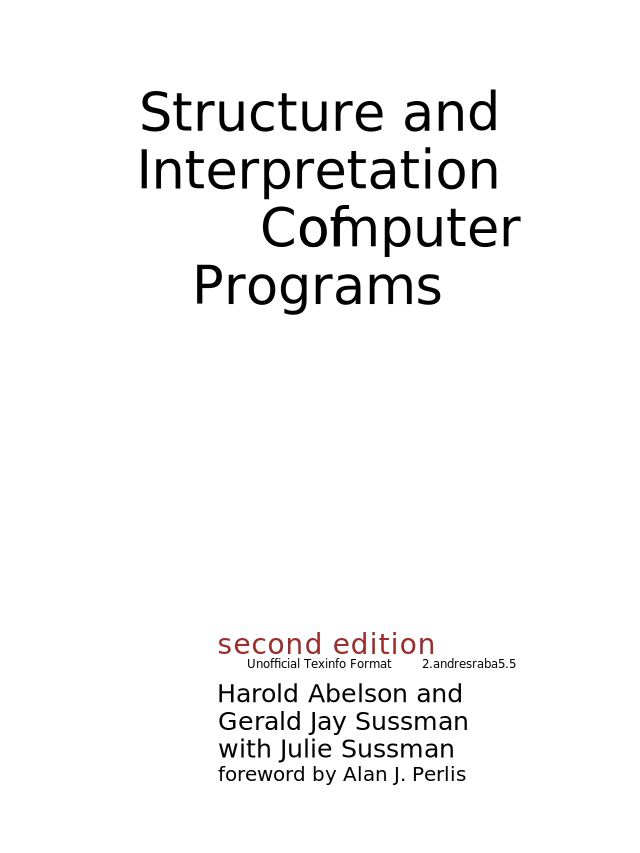
\includepdf[scale=0.92]{coverpage.pdf}

\pagebreak

\vspace*{\fill}
\thispagestyle{empty}

\begin{small}

\noindent
{\copyright}1996 by The Massachusetts Institute of Technology

\vspace{1.26em}
\noindent
Structure and Interpretation of Computer Programs,\\
second edition

\vspace{1.26em}
\noindent
Harold Abelson and Gerald Jay Sussman\\
with Julie Sussman, foreword by Alan J. Perlis

\vspace{1.6em}
\noindent
\includegraphics[width=3mm]{fig/icons/cc.pdf}
\includegraphics[width=3mm]{fig/icons/by.pdf}
\includegraphics[width=3mm]{fig/icons/sa.pdf}

\vspace{0.4em}
\noindent
This work is licensed under a Creative Commons\\ 
Attribution-ShareAlike 3.0 Unported License\\
(\href{http://creativecommons.org/licenses/by-sa/3.0/}{\acronym{CC BY-SA} 3.0}).
Based on a work at \href{http://mitpress.mit.edu/sicp/}{mitpress.mit.edu}.

\vspace{1.26em}
\noindent
The \acronym{MIT} Press\\
Cambridge, Massachusetts\\ 
London, England

\vspace{1.26em}
\noindent
McGraw-Hill Book Company\\
New York, St. Louis, San Francisco,\\ 
Montreal, Toronto

\vspace{1.26em}
\noindent
Unofficial Texinfo Format \href{http://sicpebook.wordpress.com}{2.andresraba5.2} (February 10, 2014),\\ 
based on \href{http://www.neilvandyke.org/sicp-texi/}{2.neilvandyke4} (January 10, 2007).

\end{small}

\pagebreak

\tableofcontents

\small  % Added by minghai. (Japanese fonts looks too big.)

\label{UTF}
\chapter*{Unofficial Texinfo Format}
\addcontentsline{toc}{chapter}{Unofficial Texinfo Format}

This is the second edition \acronym{SICP} book, from Unofficial Texinfo
Format.

これは\acronym{SICP}の第二版非公式Texinfo版です。

You are probably reading it in an Info hypertext browser, such as the Info
mode of Emacs.  You might alternatively be reading it {\TeX}-formatted on your
screen or printer, though that would be silly.  And, if printed, expensive.

あなたは恐らくこれをEmacsのInfoモードの様なハイパーテキストブラウザで読んで
いることでしょう。他にも{\TeX}で組版した物を画面や印刷して読んでいるかもしれませんが
それはバカバカしい上に高くつきます。

The freely-distributed official \acronym{HTML}-and-\acronym{GIF} format was
first converted personally to Unofficial Texinfo Format (\acronym{UTF})
version 1 by Lytha Ayth during a long Emacs lovefest weekend in April, 2001.

公式に無料で公開された\acronym{HTML}-and-\acronym{GIF}版を
Lytha Aythが最初に私的に、2001年4月の長いEmacs Lovefest Weekendの間に
非公式Texinfo版(\acronym{UTF})バージョン1へと変換しました。

The \acronym{UTF} is easier to search than the \acronym{HTML} format.  It is
also much more accessible to people running on modest computers, such as
donated '386-based PCs.  A 386 can, in theory, run Linux, Emacs, and a Scheme
interpreter simultaneously, but most 386s probably can't also run both Netscape
and the necessary X Window System without prematurely introducing budding young
underfunded hackers to the concept of \newterm{thrashing}.  UTF can also fit
uncompressed on a 1.44\acronym{MB} floppy diskette, which may come in handy for
installing UTF on PCs that do not have Internet or LAN access.

\acronym{UTF}はHTML版よりも検索がより簡単です。また寄付された古い386の様な
質素な計算機上で行う人々にとってよりアクセスが容易です。386は理論的にはLinux、Emacs、
Schemeインタプリタを同時に実行できます。しかし多くの386は恐らくNetscapeと必要なX Window
Systemを事前に芽の出かけた資金不足の若いハッカーに\newterm{thrashing}(スラッシング)の
概念を教えることなしに動かすことはできないでしょう。UTFはまた圧縮無しでも1.44\acronym{MB}
のフロッピーディスケットに収まります。これはインターネットやLANへの接続環境の無いPC
にインストールする場合に役立つでしょう。

The Texinfo conversion has been a straight transliteration, to the extent
possible.  Like the {\TeX}-to-\acronym{HTML} conversion, this was not without
some introduction of breakage.  In the case of Unofficial Texinfo Format,
figures have suffered an amateurish resurrection of the lost art of
\acronym{ASCII}.  Also, it's quite possible that some errors of ambiguity
were introduced during the conversion of some of the copious superscripts (`\^{}')
and subscripts (`\_').  Divining \emph{which} has been left as an exercise to
the reader. But at least we don't put our brave astronauts at risk by encoding
the \emph{greater-than-or-equal} symbol as \code{<u>\&gt;</u>}.

Texinfoへの変換は可能な範囲で直接的な翻字でした。{\TeX}-to-\acronym{HTML}変換の様に
ある程度の破れが含まれること無しにはできませんでした。非公式TexInfo形式においては
図が「失なわれた技術」であるアスキーアートによる下手糞な"復活"を被りました。また
多量の上付き文字と下付き文字のいくつかの変換の間に不明瞭さによる変換の
失敗が含まれてしまった可能性が大いにあります。読者への課題として残されたと予測します。
しかし、最低でも\emph{``以上''}の記号を\texttt{<u>\&gt;</u>}と符号化することで
我等の勇敢な宇宙飛行士を危険に置くようなことはしませんでした。

If you modify \texttt{sicp.texi} to correct errors or improve the
\acronym{ASCII} art, then update the \code{hoge}
line to reflect your delta.  For example, if you started with Lytha's version
\code{1}, and your name is Bob, then you could name your successive versions
\code{1.bob1}, \code{1.bob2}, $($ \dots \code{1.bob\textit{n}}. 

It is believed that the Unofficial Texinfo Format is in keeping with the
spirit of the graciously freely-distributed \acronym{HTML} version.  But you
never know when someone's armada of lawyers might need something to do, and get
their shorts all in a knot over some benign little thing, so think twice before
you use your full name or distribute Info, \acronym{DVI}, PostScript, or
\acronym{PDF} formats that might embed your account or machine name.

非公式Texinfo形式は寛大にも自由の下に配布された\acronym{HTML}版の魂を引き継いで
いると信じられています。しかし、いつ誰かの法律家の大艦隊が良心に基づく小さな事に対して非常に腹を立て
何かを行わなければならなくなるかもしれません。ですのであなたのフルネームを
使ったり、あなたのアカウントやマシン名を含むInfo, \acronym{DVI}, PostScript, \acronym{PDF}形式
を配布する前に良く良く考えて下さい。

\noindent
\textit{Peath,}

\noindent
\textit{Lytha Ayth}

\vspace{1.0em}
\noindent
\textbf{Addendum:} See also the \acronym{SICP} video lectures by Abelson and Sussman:\\
at \href{http://groups.csail.mit.edu/mac/classes/6.001/abelson-sussman-lectures/}{\acronym{MIT CSAIL}} or 
\href{http://ocw.mit.edu/courses/electrical-engineering-and-computer-science/6-001-structure-and-interpretation-of-computer-programs-spring-2005/video-lectures/}{\acronym{MIT OCW}}.

\textbf{付録:}AbelsonとSussmanによる\acronym{SICP}のビデオレクチャーもご覧下さい。\\
\href{http://groups.csail.mit.edu/mac/classes/6.001/abelson-sussman-lectures/}{\acronym{MIT CSAIL}}
\href{http://ocw.mit.edu/courses/electrical-engineering-and-computer-science/6-001-structure-and-interpretation-of-computer-programs-spring-2005/video-lectures/}{\acronym{MIT OCW}}.


\vspace{0.5em}
\noindent 
\textbf{Second Addendum:} Above is the original introduction to the \acronym{UTF} 
from 2001. Ten years later, \acronym{UTF} has been transformed: mathematical 
symbols and formulas are properly typeset, and figures drawn in 
vector graphics. The original text formulas and \acronym{ASCII} art figures 
are still there in the Texinfo source, but will display only when compiled 
to Info output. At the dawn of e-book readers and tablets, reading a 
\acronym{PDF} on screen is officially not silly anymore. Enjoy!

\noindent
\textbf{付録2:} 上記は2001年の元の\acronym{UTF}の紹介です。
10年後、\acronym{UTF}は一変しました。数学上の記号と式は適切に組版され、図は
ベクターグラフィックにより描かれています。元のテキスト形式とアスキーアートの図
は今でもTexinfoのソースに残っていますが、Info形式でコンパイルした場合のみ
表示されます。電子書籍リーダーとタブレットの夜明けに画面上で\acronym{PDF}を
読むことは正式に、最早バカバカしいことでは無くなりました。楽しんで下さい!

\vspace{0.5em}
\noindent
\textit{A.R, May, 2011}

\label{Chapter 1}
\chapter{手続を用いた抽象化の構築}

\pagenumbering{arabic}

\begin{quote}
The acts of the mind, wherein it exerts its power over simple ideas, are
chiefly these three: 1. Combining several simple ideas into one compound one,
and thus all complex ideas are made.  2. The second is bringing two ideas,
whether simple or complex, together, and setting them by one another so as to
take a view of them at once, without uniting them into one, by which it gets
all its ideas of relations.  3.  The third is separating them from all other
ideas that accompany them in their real existence: this is called abstraction,
and thus all its general ideas are made.

心がその力を単純な考えの上に発揮する心の働きは、主としてこれら3つです。1. いくつかの
簡単な考えを1つの複合物に組み合わせます。全ての複雑な考えはこのようにして作られます。
2. 2つ目は2つの考えをそれが簡単であるか複雑であるかに係らず一緒にもたらし、お互いに
合わせることでそれらを統合することは無しに、全ての関係性の考えを得ることで、一度に
それらを見渡します。3. 3つ目は考えをそれらの実在に付随する全ての他の考えから分離します。
これは抽象化と呼ばれ、このようにして全てのその一般的な考えは作られます。

---John Locke, \emph{An Essay Concerning Human Understanding} (1690)
\end{quote}

\vspace{1.0em}

\noindent
We are about to study the idea of a \newterm{computational process}.
Computational processes are abstract beings that inhabit computers.  As they
evolve, processes manipulate other abstract things called \newterm{data}.  The
evolution of a process is directed by a pattern of rules called a
\newterm{program}.  People create programs to direct processes.  In effect, we
conjure the spirits of the computer with our spells.

私達は\newterm{computational process}(演算プロセス)について学びます。演算プロセスとは抽象的な存在で
コンピュータ
の中に複数が住んでいます。それらが進化するとプロセスは\newterm{data}(データ)と呼ばれる
また別の抽象的な物を扱います。プロセスの進化は\newterm{program}(プログラム)と呼ばれるルールの
パターン(型、類型)により命じられます。人はプログラムを作成してプロセスに命ずるのです。
つまり私達はコンピュータの精霊に私達の呪文で魔法をかけるのです。

A computational process is indeed much like a sorcerer's idea of a spirit.  It
cannot be seen or touched.  It is not composed of matter at all.  However, it
is very real.  It can perform intellectual work.  It can answer questions.  It
can affect the world by disbursing money at a bank or by controlling a robot
arm in a factory.  The programs we use to conjure processes are like a
sorcerer's spells.  They are carefully composed from symbolic expressions in
arcane and esoteric \newterm{programming languages} that prescribe the tasks we
want our processes to perform.

演算プロセスは本当に魔法使いの精霊の考えに似ています。それは見たり触れたりは
できません。物理的な物では構成されていません。しかしとてもリアルな存在です。
知的な仕事を行います。質問にも答えます。銀行でお金を払ったり、工場でロボットの
腕をコントロールすることで世界に影響を与えることも可能です。私達が利用する
プロセスに魔法をかけるプログラムとは魔法使いの呪文のような物です。難解な秘伝の
\newterm{programming languages}(プログラミング言語)の中で記号的表現にて慎重に組み立てられプロセスに
実行してほしいタスク(仕事、任務)を指示します。

A computational process, in a correctly working computer, executes programs
precisely and accurately.  Thus, like the sorcerer's apprentice, novice
programmers must learn to understand and to anticipate the consequences of
their conjuring.  Even small errors (usually called \newterm{bugs} or
\newterm{glitches}) in programs can have complex and unanticipated
consequences.

演算プロセスは、正しく動くコンピュータでは、精密に正しくプログラムを実行します。
従って魔法使いの見習いのように、初心者のプログラマは魔法の結果について理解し、
予測することを学ばねばなりません。例えプログラムの小さなエラー
(通常は\newterm{bugs}(バグ)、または\newterm{glitches}(グリッチ、誤作動)と呼ばれます)でも
複雑で予測不可能な結果をもたらす場合もあるのです。

Fortunately, learning to program is considerably less dangerous than learning
sorcery, because the spirits we deal with are conveniently contained in a
secure way.  Real-world programming, however, requires care, expertise, and
wisdom.  A small bug in a computer-aided design program, for example, can lead
to the catastrophic collapse of an airplane or a dam or the self-destruction of
an industrial robot.

幸運なことに、プログラムを学ぶことは魔法を学ぶことより少しも危険ではありません。
私達が相手にする精霊は都合良く安全な方法で封じ込まれています。
しかし、実際の世界でのプログラミングには注意力、専門知識、堅実さを必要とします。
例えばCAD(計算機による設計支援)プログラムの小さなバグが飛行機や
ダムの最悪な崩壊に繋ったり、工業ロボットの自己破壊を起こしたりします。

Master software engineers have the ability to organize programs so that they
can be reasonably sure that the resulting processes will perform the tasks
intended.  They can visualize the behavior of their systems in advance.  They
know how to structure programs so that unanticipated problems do not lead to
catastrophic consequences, and when problems do arise, they can \newterm{debug}
their programs.  Well-designed computational systems, like well-designed
automobiles or nuclear reactors, are designed in a modular manner, so that the
parts can be constructed, replaced, and debugged separately.

ソフトウェアエンジニアのマスター達は最終的にプロセスが望まれたタスクを実行する
ことに自信を持てるだけの技能を、プログラムの構築に対して持っています。
彼らは前もってシステムの行いを図で説明することができます。予測不可能な問題が
最悪な結果をもたらさぬようプログラムをどのように構造化を行うのか知っています。
そして問題が発生した時にはプログラムの \newterm{debug}(デバッグ、バグ取り)を行えます。
良い設計のコンピュータシステムは、良い設計の自動車や原子炉のように
モジュール方式で設計されており、パーツは個別に組み立て、置き換え、デバッグが
可能です。

\subsubsection*{Lispプログラミング}

We need an appropriate language for describing processes, and we will use for
this purpose the programming language Lisp.  Just as our everyday thoughts are
usually expressed in our natural language (such as English, French, or
Japanese), and descriptions of quantitative phenomena are expressed with
mathematical notations, our procedural thoughts will be expressed in Lisp.
Lisp was invented in the late 1950s as a formalism for reasoning about the use
of certain kinds of logical expressions, called \newterm{recursion equations},
as a model for computation.  The language was conceived by John McCarthy and is
based on his paper ``Recursive Functions of Symbolic Expressions and Their
Computation by Machine'' (\link{McCarthy 1960}).

私達はプロセスを記述するのに適切な言語を必要とします。この目的に対しプログラミング
言語Lispを利用します。私達の日々の考えが通常、自然言語(例えば英語やフランス語、
日本語)で表されるように、定量的な現象が数学の記号で表されるように、手続的な
思考はLispで表現されます。Lispは1950年代後半に\newterm{recursion equations}(再帰方程式)
と呼ばれるある種の論理表現に関する推論のための形式化として開発されました。
この言語はJohn McCarthyにより着想され、彼の論文``記号式の再帰方程式とそれらの機械による演算''
(\link{McCarthy 1960})を基にしています。

Despite its inception as a mathematical formalism, Lisp is a practical
programming language.  A Lisp \newterm{interpreter} is a machine that carries
out processes described in the Lisp language.  The first Lisp interpreter was
implemented by McCarthy with the help of colleagues and students in the
Artificial Intelligence Group of the \acronym{MIT} Research Laboratory of
Electronics and in the \acronym{MIT} Computation Center.\footnote{The
\textit{Lisp 1 Programmer's Manual} appeared in 1960, and the \textit{Lisp 1.5
Programmer's Manual} (\link{McCarthy et al. 1965}) was published in 1962.  The early history
of Lisp is described in \link{McCarthy 1978}.}  Lisp, whose name is an acronym for
LISt Processing, was designed to provide symbol-manipulating capabilities for
attacking programming problems such as the symbolic differentiation and
integration of algebraic expressions.  It included for this purpose new data
objects known as atoms and lists, which most strikingly set it apart from all
other languages of the period.

数学上の形式主義としての始まりにも関わらず、Lispは実用的なプログラミング言語
です。Lisp\newterm{interpreter}(インタプリタ、逐次翻訳処理器)はLisp言語にて記述されたプロセスを実行する
機械です。最初のLispインタプリタはMcCarthyと\acronym{MIT}研究所の人工知能部門の
同僚、学生による手助けにて実装されました。\footnote{
\textit{Lisp 1 Programmer's Manual}は1960年に初出し、
\textit{Lisp 1.5 Programmer's Manual} (\link{McCarthy et al. 1965})は1962年に出版
されました。Lispの初期の歴史は\link{McCarthy 1978}にて説明されています。}
Lispはその名前をLIst Processing(リスト処理)の頭文字から取っており、
記号微分や代数式の積分の様なプログラミング上の問題に着手するための
記号操作能力を提供するために設計されました。この目的のためにアトムとリストとして
知られる新しいデータオブジェクトを含みます。これはその時代の他の全ての言語から
著しく際立たせる物でした。

Lisp was not the product of a concerted design effort.  Instead, it evolved
informally in an experimental manner in response to users' needs and to
pragmatic implementation considerations.  Lisp's informal evolution has
continued through the years, and the community of Lisp users has traditionally
resisted attempts to promulgate any ``official'' definition of the language.
This evolution, together with the flexibility and elegance of the initial
conception, has enabled Lisp, which is the second oldest language in widespread
use today (only Fortran is older), to continually adapt to encompass the most
modern ideas about program design.  Thus, Lisp is by now a family of dialects,
which, while sharing most of the original features, may differ from one another
in significant ways.  The dialect of Lisp used in this book is called
Scheme.\footnote{The two dialects in which most major Lisp programs of the
1970s were written are MacLisp (\link{Moon 1978}; \link{Pitman 1983}), developed at the
\acronym{MIT} Project \acronym{MAC}, and Interlisp (\link{Teitelman 1974}), developed
at Bolt Beranek and Newman Inc. and the Xerox Palo Alto Research Center.
Portable Standard Lisp (\link{Hearn 1969}; \link{Griss 1981}) was a Lisp dialect designed to
be easily portable between different machines.  MacLisp spawned a number of
subdialects, such as Franz Lisp, which was developed at the University of
California at Berkeley, and Zetalisp (\link{Moon and Weinreb 1981}), which was based on a
special-purpose processor designed at the \acronym{MIT} Artificial Intelligence
Laboratory to run Lisp very efficiently.  The Lisp dialect used in this book,
called Scheme (\link{Steele and Sussman 1975}), was invented in 1975 by Guy Lewis Steele Jr. and
Gerald Jay Sussman of the \acronym{MIT} Artificial Intelligence Laboratory and
later reimplemented for instructional use at \acronym{MIT}.  Scheme became an
\acronym{IEEE} standard in 1990 (\link{IEEE 1990}).  The Common Lisp dialect
(\link{Steele 1982}, \link{Steele 1990}) was developed by the Lisp community to combine
features from the earlier Lisp dialects to make an industrial standard for
Lisp.  Common Lisp became an \acronym{ANSI} standard in 1994 (\link{ANSI 1994}).}

Lispは計画的な設計の取り組みから生まれた製品ではありませんでした。そうではなく、
非公式に試験的なやり方で、ユーザの要求と実利的な実装上の考慮への対応として発展しました。
Lispの非公式な進化は何年も続き、Lispユーザのコミュニティは伝統的に言語の``公式な''
どんな定義の公表に対しても抵抗しました。この進化は初期構想の柔軟性と洗練さと共に、今日
世界中で広く使用される言語で2番目に古い(Fortranのみがより古い)言語として、Lispに継続的に
最新のプログラム設計についての考えを受け入れることを可能にしてきました。
従ってLispは今では複数の方言の系統が存在し、それらはオリジナルの機能の多くを共有しながらも、
お互いに大きな違いを持ちます。この本で使用されるLispの方言はSchemeと呼ばれます。\footnote{
1970年代に最もメジャーなLispプログラムの記述に用いられた2つの方言は\acronym{MIT}のプロジェクト
\acronym{MAC}で開発されたMacLisp (\link{Moon 1978}; \link{Pitman 1983})と
Bolt Beranek and Newman Inc.とXerox Palo Alto研究センターににて開発された
Interlisp (\link{Teitelman 1974})でした。Portable Standard Lisp (\link{Hearn 1969}; \link{Griss 1981})
は簡単に、異なるマシンの間で移植可能にするよう設計されたLisp方言です。MacLispは
カリフォルニア大学バークレー校により開発されたFranz Lispや\acronym{MIT}人口知能研究所が
Lispをとても効率良く実行するために設計した特定目的プロセッサ(処理機)をベースにした
Zetalisp (\link{Moon and Weinreb 1981})といったいくつかの下位方言を生みました。
この本で使用するLisp方言はSheme (\link{Steele and Sussman 1975})と呼ばれ、1975年に
\acronym{MIT}人口知能研究所のGuy Lewis Steele Jr.とGerald Jay Sussmanにより開発され、
後に\acronym{MIT}にて教育目的のために再実装されました。
Common Lisp (\link{Steele 1982}, \link{Steele 1990})はLispコミュニティにより初期のLisp方言の
機能を集約し、Lispの業界標準を作成するために開発されました。Common Lispは1994年に
\acronym{ANSI}標準(\link{ANSI 1994})になりました。
}

Because of its experimental character and its emphasis on symbol manipulation,
Lisp was at first very inefficient for numerical computations, at least in
comparison with Fortran.  Over the years, however, Lisp compilers have been
developed that translate programs into machine code that can perform numerical
computations reasonably efficiently.  And for special applications, Lisp has
been used with great effectiveness.\footnote{One such special application was a
breakthrough computation of scientific importance---an integration of the
motion of the Solar System that extended previous results by nearly two orders
of magnitude, and demonstrated that the dynamics of the Solar System is
chaotic.  This computation was made possible by new integration algorithms, a
special-purpose compiler, and a special-purpose computer all implemented with
the aid of software tools written in Lisp (\link{Abelson et al. 1992}; \link{Sussman and Wisdom 1992}).}  
Although Lisp has not yet overcome its old reputation as
hopelessly inefficient, Lisp is now used in many applications where efficiency
is not the central concern.  For example, Lisp has become a language of choice
for operating-system shell languages and for extension languages for editors
and computer-aided design systems.

実験的であるという特徴と記号操作の重要性のため、Lispは初期においては数値演算に対し
少くともFortranとの比較にてとても非効率でした。しかし年を追って、プログラムを
機械語に変換し、数値演算を適度に効率良く実行可能なLispコンパイラが開発されました。
特別なアプリケーションに対してはLispは最高の効果を発揮しています。\footnote{
そのような特別なアプリケーションの1つは自然科学上の重大な計算、太陽系の動きの統合
におけるブレイクスルーでした。これは以前の結果より二桁も良く、太陽系の活動が混沌
であることを実演しました。この計算は全てLispで書かれたソフトウェアツールの手助け
により実装された新しい統合アルゴリズム、特定目的のコンパイラ、特定目的の計算機に
より可能となりました。(\link{Abelson et al. 1992}; \link{Sussman and Wisdom 1992})}
Lispは今でもどうしようもなく非効率であるという古い評判を乗り越えられてはいませんが、
Lispは今では多くのアプリケーションにて、効率が問題の中心ではない場合において
利用されています。例えばLispはOSのシェル言語やエディタの拡張言語、CADシステム等に
おいて選択言語となっています。

If Lisp is not a mainstream language, why are we using it as the framework for
our discussion of programming?  Because the language possesses unique features
that make it an excellent medium for studying important programming constructs
and data structures and for relating them to the linguistic features that
support them.  The most significant of these features is the fact that Lisp
descriptions of processes, called \newterm{procedures}, can themselves be
represented and manipulated as Lisp data.  The importance of this is that there
are powerful program-design techniques that rely on the ability to blur the
traditional distinction between ``passive'' data and ``active'' processes.  As
we shall discover, Lisp's flexibility in handling procedures as data makes it
one of the most convenient languages in existence for exploring these
techniques.  The ability to represent procedures as data also makes Lisp an
excellent language for writing programs that must manipulate other programs as
data, such as the interpreters and compilers that support computer languages.
Above and beyond these considerations, programming in Lisp is great fun.

もしLispがメインストリームの言語でなければなぜ私達はプログラミングの議論のための
フレームワークとしてそれを用いるのでしょうか? なぜならこの言語は
重要なプログラミング構成概念とデータ構造を学ぶため、またそれらをサポートする
言語上の機能にそれらを関連付けするために、言語自身を洗練された媒体と成す個有の機能
を持っているためです。
これらの機能で最も著しい物は、Lispによる\newterm{procedures}(プロシジャ、手続)と
呼ばれるプロセスの記述が、それ自身がLispのデータとして表現され、また操作されることが可能
であるという事実です。これの重要性は、伝統的な``受動的な''データと``能動的な''
プロセスとの間の区別をぼかす能力に依存する、強力なプログラム設計のテクニックが存在する
ということです。私達がそれを発見するにつれ、手続をデータとして扱うLispの柔軟性は
Lispをこれらのテクニックを探求するのに、既存で最も便利な言語の1つとします。
手続をデータとして表現する能力はまた、Lispを他のプログラムをデータとして操作しなければ
ならないプログラムを書く目的に対し洗練された言語にします。例えばコンピュータ言語に
対応するインタプリタやコンパイラのようなプログラムです。これらの考慮点に加えて、
Lispによるプログラミングはとても楽しいのです。



\label{Section 1.1}
\section{The Elements of Programming}

A powerful programming language is more than just a means for instructing a
computer to perform tasks.  The language also serves as a framework within
which we organize our ideas about processes.  Thus, when we describe a
language, we should pay particular attention to the means that the language
provides for combining simple ideas to form more complex ideas.  Every powerful
language has three mechanisms for accomplishing this:

強力なプログラミング言語はコンピュータにタスクの実行を指示するだけではありません。
そのような言語は私達がプロセスについての自らの考えを体系化するフレームワークとして
の役目を担います。従って言語を記述する時、簡単なアイデアを組み合わせてより複雑な
アイデアを形成するという手段をその言語が提供することには特に注意を払わねばなりません。
強力な言語全てがこれを達成するために3つのメカニズムを持っています。

\chapter*{References}
\addcontentsline{toc}{chapter}{References}
\label{References}

\phantomsection \label{Abelson et al. 1992}
Abelson, Harold, Andrew Berlin, Jacob Katzenelson, William McAllister,
Guillermo Rozas, Gerald Jay Sussman, and Jack Wisdom. 1992.  The Supercomputer
Toolkit: A general framework for special-purpose computing.
\textit{International Journal of High-Speed Electronics} 3(3): 337-361.
\href{http://www.hpl.hp.com/techreports/94/HPL-94-30.html}{\code{(Onl)}}

\phantomsection \label{Allen 1978}
Allen, John.  1978.  \textit{Anatomy of Lisp}. New York: McGraw-Hill.

\phantomsection \label{ANSI 1994}
\acronym{ANSI} X3.226-1994. \textit{American National Standard for Information
Sys\-tems---Programming Language---Common Lisp}.

\phantomsection \label{Appel 1987}
Appel, Andrew W.  1987.  Garbage collection can be faster than stack
allocation.  \textit{Information Processing Letters} 25(4): 275-279.
\href{http://citeseer.ist.psu.edu/viewdoc/summary?doi=10.1.1.39.8219}{\code{(Online)}}

\phantomsection \label{Backus 1978}
Backus, John.  1978.  Can programming be liberated from the von Neumann style?
\textit{Communications of the \acronym{ACM}} 21(8): 613-641.
\href{http://www.stanford.edu/class/cs242/readings/backus.pdf}{\code{(Online)}}

\phantomsection \label{Baker (1978)}
Baker, Henry G., Jr.  1978.  List processing in real time on a serial computer.
\textit{Communications of the \acronym{ACM}} 21(4): 280-293.
\href{http://dspace.mit.edu/handle/1721.1/41976}{\code{(Online)}}

\phantomsection \label{Batali et al. 1982}
Batali, John, Neil Mayle, Howard Shrobe, Gerald Jay Sussman, and Daniel Weise.
1982.  The Scheme-81 architecture---System and chip.  In \textit{Proceedings of
the \acronym{MIT} Conference on Advanced Research in \acronym{VLSI}}, edited by
Paul Penfield, Jr. Dedham, MA: Artech House.

\phantomsection \label{Borning (1977)}
Borning, Alan.  1977.  ThingLab---An object-oriented system for building
simulations using constraints. In \textit{Proceedings of the 5th International
Joint Conference on Artificial Intelligence}.
\href{http://ijcai.org/Past\%20Proceedings/IJCAI-77-VOL1/PDF/085.pdf}{\code{(Online)}}

\phantomsection \label{Borodin and Munro (1975)}
Borodin, Alan, and Ian Munro.  1975.  \textit{The Computational Complexity of
Algebraic and Numeric Problems}. New York: American Elsevier.

\phantomsection \label{Chaitin 1975}
Chaitin, Gregory J.  1975.  Randomness and mathematical proof.
\textit{Scientific American} 232(5): 47-52.

\phantomsection \label{Church (1941)}
Church, Alonzo.  1941.  \textit{The Calculi of Lambda-Conversion}.  Princeton,
N.J.: Princeton University Press.

\phantomsection \label{Clark (1978)}
Clark, Keith L.  1978.  Negation as failure.  In \textit{Logic and Data Bases}.
New York: Plenum Press, pp. 293-322.
\href{http://www.doc.ic.ac.uk/~klc/neg.html}{\code{(Online)}}

\phantomsection \label{Clinger (1982)}
Clinger, William.  1982.  Nondeterministic call by need is neither lazy nor by
name. In \textit{Proceedings of the \acronym{ACM} Symposium on Lisp and
Functional Programming}, pp. 226-234.

\phantomsection \label{Clinger and Rees 1991}
Clinger, William, and Jonathan Rees.  1991.  Macros that work.  In
\textit{Proceedings of the 1991 \acronym{ACM} Conference on Principles of
Programming Languages}, pp. 155-162.
\href{http://mumble.net/~jar/pubs/macros_that_work.ps}{\code{(Online)}}

\phantomsection \label{Colmerauer et al. 1973}
Colmerauer A., H. Kanoui, R. Pasero, and P. Roussel.  1973.  Un syst\`eme de
communication homme-machine en fran\c{c}ais.  Technical report, Groupe
Intelligence Artificielle, Universit\'e d'Aix Marseille, Luminy.

\phantomsection \label{Cormen et al. 1990}
Cormen, Thomas, Charles Leiserson, and Ronald Rivest.  1990. \textit{Introduction
to Algorithms}. Cambridge, MA: \acronym{MIT} Press.

\phantomsection \label{Darlington et al. 1982}
Darlington, John, Peter Henderson, and David Turner.  1982.  \textit{Functional
Programming and Its Applications}. New York: Cambridge University Press.

\phantomsection \label{Dijkstra 1968a}
Dijkstra, Edsger W. 1968a.  The structure of the ``\acronym{THE}''
multiprogramming system.  \textit{Communications of the \acronym{ACM}}
11(5): 341-346.
\href{http://www.cs.utexas.edu/users/EWD/ewd01xx/EWD196.PDF}{\code{(Online)}}

\phantomsection \label{Dijkstra 1968b}
Dijkstra, Edsger W. 1968b.  Cooperating sequential processes.  In
\textit{Programming Languages}, edited by F. Genuys. New York: Academic Press,
pp.  43-112.
\href{http://www.cs.utexas.edu/users/EWD/ewd01xx/EWD123.PDF}{\code{(Online)}}

\phantomsection \label{Dinesman 1968}
Dinesman, Howard P.  1968.  \textit{Superior Mathematical Puzzles}.  New York:
Simon and Schuster.

\phantomsection \label{deKleer et al. 1977}
deKleer, Johan, Jon Doyle, Guy Steele, and Gerald J. Sussman.  1977.
\acronym{AMORD}: Explicit control of reasoning.  In \textit{Proceedings of the
\acronym{ACM} Symposium on Artificial Intelligence and Programming Languages},
pp.  116-125.
\href{http://dspace.mit.edu/handle/1721.1/5750}{\code{(Online)}}

\phantomsection \label{Doyle (1979)}
Doyle, Jon. 1979. A truth maintenance system. \textit{Artificial Intelligence}
12: 231-272.
\href{http://dspace.mit.edu/handle/1721.1/5733}{\code{(Online)}}

\phantomsection \label{Feigenbaum and Shrobe 1993}
Feigenbaum, Edward, and Howard Shrobe. 1993. The Japanese National Fifth
Generation Project: Introduction, survey, and evaluation.  In \textit{Future
Generation Computer Systems}, vol. 9, pp. 105-117.

\phantomsection \label{Feeley (1986)}
Feeley, Marc.  1986.  Deux approches \`a l'implantation du language
Scheme.  Masters thesis, Universit\'e de Montr\'eal.

\phantomsection \label{Feeley and Lapalme 1987}
Feeley, Marc and Guy Lapalme.  1987.  Using closures for code generation.
\textit{Journal of Computer Languages} 12(1): 47-66.
\href{http://citeseerx.ist.psu.edu/viewdoc/summary?doi=10.1.1.90.6978}{\code{(Online)}}

Feller, William.  1957.  \textit{An Introduction to Probability Theory and Its
Applications}, volume 1. New York: John Wiley \& Sons.

\phantomsection \label{Fenichel and Yochelson (1969)}
Fenichel, R., and J. Yochelson.  1969.  A Lisp garbage collector for virtual
memory computer systems.  \textit{Communications of the \acronym{ACM}}
12(11): 611-612.

\phantomsection \label{Floyd (1967)}
Floyd, Robert. 1967. Nondeterministic algorithms. \textit{\acronym{JACM}},
14(4): 636-644.

\phantomsection \label{Forbus and deKleer 1993}
Forbus, Kenneth D., and Johan deKleer.  1993. \textit{Building Problem
Solvers}. Cambridge, MA: \acronym{MIT} Press.

\phantomsection \label{Friedman and Wise (1976)}
Friedman, Daniel P., and David S. Wise.  1976.  \acronym{CONS} should not
evaluate its arguments. In \textit{Automata, Languages, and Programming: Third
International Colloquium}, edited by S. Michaelson and R.  Milner, pp. 257-284.
\href{https://www.cs.indiana.edu/cgi-bin/techreports/TRNNN.cgi?trnum=TR44}{\code{(Online)}}

\phantomsection \label{Friedman et al. 1992}
Friedman, Daniel P., Mitchell Wand, and Christopher T. Haynes. 1992.
\textit{Essentials of Programming Languages}.  Cambridge, MA: \acronym{MIT}
Press/ McGraw-Hill.

\phantomsection \label{Gabriel 1988}
Gabriel, Richard P. 1988.  The Why of \emph{Y}.  \textit{Lisp Pointers}
2(2): 15-25.
\href{http://www.dreamsongs.com/Files/WhyOfY.pdf}{\code{(Online)}}

Goldberg, Adele, and David Robson.  1983.  \textit{Smalltalk-80: The Language and
Its Implementation}. Reading, MA: Addison-Wesley.

\phantomsection \label{Gordon et al. 1979}
Gordon, Michael, Robin Milner, and Christopher Wadsworth.  1979.
\textit{Edinburgh LCF}. Lecture Notes in Computer Science, volume 78. New York:
Springer-Verlag.

\phantomsection \label{Gray and Reuter 1993}
Gray, Jim, and Andreas Reuter. 1993. \textit{Transaction Processing: Concepts and
Models}. San Mateo, CA: Morgan-Kaufman.

\phantomsection \label{Green 1969}
Green, Cordell.  1969.  Application of theorem proving to problem solving.  In
\textit{Proceedings of the International Joint Conference on Artificial
Intelligence}, pp. 219-240.
\href{http://citeseer.ist.psu.edu/viewdoc/summary?doi=10.1.1.81.9820}{\code{(Online)}}

\phantomsection \label{Green and Raphael (1968)}
Green, Cordell, and Bertram Raphael.  1968.  The use of theorem-proving
techniques in question-answering systems.  In \textit{Proceedings of the
\acronym{ACM} National Conference}, pp. 169-181.

\phantomsection \label{Griss 1981}
Griss, Martin L.  1981.  Portable Standard Lisp, a brief overview.  Utah
Symbolic Computation Group Operating Note 58, University of Utah.

\phantomsection \label{Guttag 1977}
Guttag, John V.  1977.  Abstract data types and the development of data
structures.  \textit{Communications of the \acronym{ACM}} 20(6): 396-404.
\href{http://www.unc.edu/~stotts/comp723/guttagADT77.pdf}{\code{(Online)}}

\phantomsection \label{Hamming 1980}
Hamming, Richard W.  1980.  \textit{Coding and Information Theory}.  Englewood
Cliffs, N.J.: Prentice-Hall.

\phantomsection \label{Hanson 1990}
Hanson, Christopher P.  1990.  Efficient stack allocation for tail-recur\-sive
languages.  In \textit{Proceedings of \acronym{ACM} Conference on Lisp and
Functional Programming}, pp. 106-118.

\phantomsection \label{Hanson 1991}
Hanson, Christopher P.  1991.  A syntactic closures macro facility.  \textit{Lisp
Pointers}, 4(3).
\href{http://groups.csail.mit.edu/mac/ftpdir/scheme-reports/synclo.ps}{\code{(Online)}}

\phantomsection \label{Hardy 1921}
Hardy, Godfrey H.  1921.  Srinivasa Ramanujan.  \textit{Proceedings of the London
Mathematical Society} XIX(2).

\phantomsection \label{Hardy and Wright 1960}
Hardy, Godfrey H., and E. M. Wright.  1960.  \textit{An Introduction to the
Theory of Numbers}.  4th edition.  New York: Oxford University Press.

\phantomsection \label{Havender (1968)}
Havender, J. 1968. Avoiding deadlocks in multi-tasking systems. \textit{IBM
Systems Journal} 7(2): 74-84.

\phantomsection \label{Hearn 1969}
Hearn, Anthony C.  1969.  Standard Lisp.  Technical report \acronym{AIM}-90,
Artificial Intelligence Project, Stanford University.
\href{http://www.softwarepreservation.org/projects/LISP/stanford/Hearn-StandardLisp-AIM-90.pdf}{\code{(Online)}}

\phantomsection \label{Henderson 1980}
Henderson, Peter. 1980.  \textit{Functional Programming: Application and
Implementation}. Englewood Cliffs, N.J.: Prentice-Hall.

\phantomsection \label{Henderson 1982}
Henderson. Peter. 1982. Functional Geometry. In \textit{Conference Record of the
1982 \acronym{ACM} Symposium on Lisp and Functional Programming}, pp. 179-187.
\href{http://pmh-systems.co.uk/phAcademic/papers/funcgeo.pdf}{\code{(Online)}}
\href{http://eprints.soton.ac.uk/257577/1/funcgeo2.pdf}{\code{(2002 version)}}

\phantomsection \label{Hewitt (1969)}
Hewitt, Carl E.  1969.  \acronym{PLANNER}: A language for proving
theorems in robots.  In \textit{Proceedings of the International Joint
Conference on Artificial Intelligence}, pp. 295-301.
\href{http://dspace.mit.edu/handle/1721.1/6171}{\code{(Online)}}

\phantomsection \label{Hewitt (1977)}
Hewitt, Carl E.  1977.  Viewing control structures as patterns of passing
messages.  \textit{Journal of Artificial Intelligence} 8(3): 323-364.
\href{http://dspace.mit.edu/handle/1721.1/6272}{\code{(Online)}}

\phantomsection \label{Hoare (1972)}
Hoare, C. A. R. 1972.  Proof of correctness of data representations.
\textit{Acta Informatica} 1(1).

\phantomsection \label{Hodges 1983}
Hodges, Andrew. 1983.  \textit{Alan Turing: The Enigma}. New York: Simon and
Schuster.

\phantomsection \label{Hofstadter 1979}
Hofstadter, Douglas R.  1979.  \textit{G\"odel, Escher, Bach: An Eternal Golden
Braid}. New York: Basic Books.

\phantomsection \label{Hughes 1990}
Hughes, R. J. M.  1990.  Why functional programming matters.  In \textit{Research
Topics in Functional Programming}, edited by David Turner.  Reading, MA:
Addison-Wesley, pp. 17-42.
\href{http://www.cs.kent.ac.uk/people/staff/dat/miranda/whyfp90.pdf}{\code{(Online)}}

\phantomsection \label{IEEE 1990}
\acronym{IEEE} Std 1178-1990.  1990.  \textit{\acronym{IEEE} Standard for the
Scheme Programming Language}.

\phantomsection \label{Ingerman et al. 1960}
Ingerman, Peter, Edgar Irons, Kirk Sattley, and Wallace Feurzeig; assisted by
M. Lind, Herbert Kanner, and Robert Floyd.  1960.  \acronym{THUNKS}: A way of
compiling procedure statements, with some comments on procedure declarations.
Unpublished manuscript.  (Also, private communication from Wallace Feurzeig.)

\phantomsection \label{Kaldewaij 1990}
Kaldewaij, Anne. 1990.  \textit{Programming: The Derivation of Algorithms}. New
York: Prentice-Hall.

\phantomsection \label{Knuth (1973)}
Knuth, Donald E.  1973.  \textit{Fundamental Algorithms}. Volume 1 of \textit{The
Art of Computer Programming}.  2nd edition. Reading, MA: Addison-Wesley.

\phantomsection \label{Knuth 1981}
Knuth, Donald E.  1981.  \textit{Seminumerical Algorithms}. Volume 2 of \textit{The
Art of Computer Programming}.  2nd edition. Reading, MA: Addison-Wesley.

\phantomsection \label{Kohlbecker 1986}
Kohlbecker, Eugene Edmund, Jr. 1986.  Syntactic extensions in the programming
language Lisp.  Ph.D. thesis, Indiana University.
\href{http://www.ccs.neu.edu/scheme/pubs/dissertation-kohlbecker.pdf}{\code{(Online)}}

\phantomsection \label{Konopasek and Jayaraman 1984}
Konopasek, Milos, and Sundaresan Jayaraman.  1984.  \textit{The TK!Solver Book: A
Guide to Problem-Solving in Science, Engineering, Business, and
Education}. Berkeley, CA: Osborne/McGraw-Hill.

\phantomsection \label{Kowalski (1973; 1979)}
Kowalski, Robert.  1973.  Predicate logic as a programming language.  Technical
report 70, Department of Computational Logic, School of Artificial
Intelligence, University of Edinburgh.
\href{http://www.doc.ic.ac.uk/~rak/papers/IFIP\%2074.pdf}{\code{(Online)}}

Kowalski, Robert.  1979.  \textit{Logic for Problem Solving}. New York:
North-Holland.

\phantomsection \label{Lamport (1978)}
Lamport, Leslie. 1978.  Time, clocks, and the ordering of events in a
distributed system.  \textit{Communications of the \acronym{ACM}} 21(7): 558-565.
\href{http://www.stanford.edu/class/cs240/readings/lamport.pdf}{\code{(Online)}}

\phantomsection \label{Lampson et al. 1981}
Lampson, Butler, J. J. Horning, R.  London, J. G. Mitchell, and G. K.  Popek.
1981.  Report on the programming language Euclid.  Technical report, Computer
Systems Research Group, University of Toronto.
\href{http://www.bitsavers.org/pdf/xerox/parc/techReports/CSL-81-12_Report_On_The_Programming_Language_Euclid.pdf}{\code{(Online)}}

\phantomsection \label{Landin (1965)}
Landin, Peter.  1965.  A correspondence between Algol 60 and Church's lambda
notation: Part I.  \textit{Communications of the \acronym{ACM}} 8(2): 89-101.

\phantomsection \label{Lieberman and Hewitt 1983}
Lieberman, Henry, and Carl E. Hewitt. 1983. A real-time garbage collector based
on the lifetimes of objects. \textit{Communications of the \acronym{ACM}}
26(6): 419-429.
\href{http://dspace.mit.edu/handle/1721.1/6335}{\code{(Online)}}

\phantomsection \label{Liskov and Zilles (1975)}
Liskov, Barbara H., and Stephen N. Zilles.  1975.  Specification techniques for
data abstractions.  \textit{\acronym{IEEE} Transactions on Software Engineering}
1(1): 7-19.
\href{http://csg.csail.mit.edu/CSGArchives/memos/Memo-117.pdf}{\code{(Online)}}

\phantomsection \label{McAllester (1978; 1980)}
McAllester, David Allen.  1978.  A three-valued truth-maintenance system.  Memo
473, \acronym{MIT} Artificial Intelligence Laboratory.
\href{http://dspace.mit.edu/handle/1721.1/6296}{\code{(Online)}}

McAllester, David Allen.  1980.  An outlook on truth maintenance.  Memo 551,
\acronym{MIT} Artificial Intelligence Laboratory.
\href{http://dspace.mit.edu/handle/1721.1/6327}{\code{(Online)}}

\phantomsection \label{McCarthy 1960}
McCarthy, John.  1960.  Recursive functions of symbolic expressions and their
computation by machine.  \textit{Communications of the \acronym{ACM}}
3(4): 184-195.
\href{http://innovation.it.uts.edu.au/projectjmc/articles/recursive.html}{\code{(Online)}}

\phantomsection \label{McCarthy 1963}
McCarthy, John.  1963.  A basis for a mathematical theory of computation.  In
\textit{Computer Programming and Formal Systems}, edited by P. Braffort and
D. Hirschberg.  North-Holland.
\href{http://innovation.it.uts.edu.au/projectjmc/articles/basis.html}{\code{(Online)}}

\phantomsection \label{McCarthy 1978}
McCarthy, John.  1978.  The history of Lisp.  In \textit{Proceedings of the
\acronym{ACM} \acronym{SIGPLAN} Conference on the History of Programming
Languages}.
\href{http://innovation.it.uts.edu.au/projectjmc/articles/lisp.html}{\code{(Online)}}

\phantomsection \label{McCarthy et al. 1965}
McCarthy, John, P. W. Abrahams, D. J. Edwards, T. P. Hart, and M. I.  Levin.
1965.  \textit{Lisp 1.5 Programmer's Manual}.  2nd edition.  Cambridge, MA:
\acronym{MIT} Press.
\href{http://www.softwarepreservation.org/projects/LISP/book/LISP\%201.5\%20Programmers\%20Manual.pdf/view}{\code{(Online)}}

\phantomsection \label{McDermott and Sussman (1972)}
McDermott, Drew, and Gerald Jay Sussman.  1972. Conniver reference manual.
Memo 259, \acronym{MIT} Artificial Intelligence Laboratory.
\href{http://dspace.mit.edu/handle/1721.1/6203}{\code{(Online)}}

\phantomsection \label{Miller 1976}
Miller, Gary L.  1976.  Riemann's Hypothesis and tests for primality.
\textit{Journal of Computer and System Sciences} 13(3): 300-317.
\href{http://www.cs.cmu.edu/~glmiller/Publications/b2hd-Mi76.html}{\code{(Online)}}

\phantomsection \label{Miller and Rozas 1994}
Miller, James S., and Guillermo J. Rozas. 1994.  Garbage collection is fast,
but a stack is faster.  Memo 1462, \acronym{MIT} Artificial Intelligence
Laboratory.
\href{http://dspace.mit.edu/handle/1721.1/6622}{\code{(Online)}}

\phantomsection \label{Moon 1978}
Moon, David.  1978.  MacLisp reference manual, Version 0.  Technical report,
\acronym{MIT} Laboratory for Computer Science.
\href{http://www.softwarepreservation.org/projects/LISP/MIT/Moon-MACLISP_Reference_Manual-Apr_08_1974.pdf/view}{\code{(Online)}}

\phantomsection \label{Moon and Weinreb 1981}
Moon, David, and Daniel Weinreb.  1981.  Lisp machine manual.  Technical
report, \acronym{MIT} Artificial Intelligence Laboratory.
\href{http://www.unlambda.com/lmman/index.html}{\code{(Online)}}

\phantomsection \label{Morris et al. 1980}
Morris, J. H., Eric Schmidt, and Philip Wadler.  1980.  Experience with an
applicative string processing language.  In \textit{Proceedings of the 7th Annual
\acronym{ACM} \acronym{SIGACT}/\acronym{SIGPLAN} Symposium on the Principles of
Programming Languages}.

\phantomsection \label{Phillips 1934}
Phillips, Hubert.  1934. \textit{The Sphinx Problem Book}.  London: Faber and
Faber.

\phantomsection \label{Pitman 1983}
Pitman, Kent. 1983. The revised MacLisp Manual (Saturday evening edition).
Technical report 295, \acronym{MIT} Laboratory for Computer Science.
\href{http://maclisp.info/pitmanual}{\code{(Online)}}

\phantomsection \label{Rabin 1980}
Rabin, Michael O. 1980. Probabilistic algorithm for testing primality.
\textit{Journal of Number Theory} 12: 128-138.

\phantomsection \label{Raymond 1993}
Raymond, Eric.  1993. \textit{The New Hacker's Dictionary}. 2nd edition.
Cambridge, MA: \acronym{MIT} Press.
\href{http://www.outpost9.com/reference/jargon/jargon_toc.html}{\code{(Online)}}

Raynal, Michel. 1986. \textit{Algorithms for Mutual Exclusion}.  Cambridge, MA:
\acronym{MIT} Press.

\phantomsection \label{Rees and Adams 1982}
Rees, Jonathan A., and Norman I. Adams IV. 1982.  T: A dialect of Lisp or,
lambda: The ultimate software tool.  In \textit{Conference Record of the 1982
\acronym{ACM} Symposium on Lisp and Functional Programming}, pp.  114-122.
\href{http://people.csail.mit.edu/riastradh/t/adams82t.pdf}{\code{(Online)}}

Rees, Jonathan, and William Clinger (eds). 1991.  The \( \rm revised^4 \) report on the
algorithmic language Scheme.  \textit{Lisp Pointers}, 4(3).
\href{http://people.csail.mit.edu/jaffer/r4rs_toc.html}{\code{(Online)}}

\phantomsection \label{Rivest et al. (1977)}
Rivest, Ronald, Adi Shamir, and Leonard Adleman.  1977.  A method for obtaining
digital signatures and public-key cryptosystems. Technical memo LCS/TM82,
\acronym{MIT} Laboratory for Computer Science.
\href{http://people.csail.mit.edu/rivest/Rsapaper.pdf}{\code{(Online)}}

\phantomsection \label{Robinson 1965}
Robinson, J. A. 1965.  A machine-oriented logic based on the resolution
principle.  \textit{Journal of the \acronym{ACM}} 12(1): 23.

\phantomsection \label{Robinson 1983}
Robinson, J. A. 1983.  Logic programming---Past, present, and future.
\textit{New Generation Computing} 1: 107-124.

\phantomsection \label{Spafford 1989}
Spafford, Eugene H.  1989.  The Internet Worm: Crisis and aftermath.
\textit{Communications of the \acronym{ACM}} 32(6): 678-688.
\href{http://citeseerx.ist.psu.edu/viewdoc/download?doi=10.1.1.123.8503&rep=rep1&type=pdf}{\code{(Online)}}

\phantomsection \label{Steele 1977}
Steele, Guy Lewis, Jr.  1977.  Debunking the ``expensive procedure call'' myth.
In \textit{Proceedings of the National Conference of the \acronym{ACM}},
pp. 153-62.
\href{http://dspace.mit.edu/handle/1721.1/5753}{\code{(Online)}}

\phantomsection \label{Steele 1982}
Steele, Guy Lewis, Jr.  1982.  An overview of Common Lisp.  In
\textit{Proceedings of the \acronym{ACM} Symposium on Lisp and Functional
Programming}, pp. 98-107.

\phantomsection \label{Steele 1990}
Steele, Guy Lewis, Jr.  1990.  \textit{Common Lisp: The Language}. 2nd edition.
Digital Press.
\href{http://www.cs.cmu.edu/Groups/AI/html/cltl/cltl2.html}{\code{(Online)}}

\phantomsection \label{Steele and Sussman 1975}
Steele, Guy Lewis, Jr., and Gerald Jay Sussman.  1975.  Scheme: An interpreter
for the extended lambda calculus.  Memo 349, \acronym{MIT} Artificial
Intelligence Laboratory.
\href{http://dspace.mit.edu/handle/1721.1/5794}{\code{(Online)}}

\phantomsection \label{Steele et al. 1983}
Steele, Guy Lewis, Jr., Donald R. Woods, Raphael A. Finkel, Mark R.  Crispin,
Richard M. Stallman, and Geoffrey S. Goodfellow.  1983.  \textit{The Hacker's
Dictionary}. New York: Harper \& Row.
\href{http://www.dourish.com/goodies/jargon.html}{\code{(Online)}}

\phantomsection \label{Stoy 1977}
Stoy, Joseph E.  1977.  \textit{Denotational Semantics}. Cambridge, MA:
\acronym{MIT} Press.

\phantomsection \label{Sussman and Stallman 1975}
Sussman, Gerald Jay, and Richard M. Stallman.  1975.  Heuristic techniques in
computer-aided circuit analysis.  \textit{\acronym{IEEE} Transactions on Circuits
and Systems} CAS-22(11): 857-865.
\href{http://dspace.mit.edu/handle/1721.1/5803}{\code{(Online)}}

\phantomsection \label{Sussman and Steele 1980}
Sussman, Gerald Jay, and Guy Lewis Steele Jr.  1980.  Constraints---A language
for expressing almost-hierachical descriptions.  \textit{AI Journal} 14: 1-39.
\href{http://dspace.mit.edu/handle/1721.1/6312}{\code{(Online)}}

\phantomsection \label{Sussman and Wisdom 1992}
Sussman, Gerald Jay, and Jack Wisdom.  1992. Chaotic evolution of the solar
system.  \textit{Science} 257: 256-262.
\href{http://groups.csail.mit.edu/mac/users/wisdom/ss-chaos.pdf}{\code{(Online)}}

\phantomsection \label{Sussman et al. (1971)}
Sussman, Gerald Jay, Terry Winograd, and Eugene Charniak.  1971.  Microplanner
reference manual.  Memo 203A, \acronym{MIT} Artificial Intelligence Laboratory.
\href{http://dspace.mit.edu/handle/1721.1/6184}{\code{(Online)}}

\phantomsection \label{Sutherland (1963)}
Sutherland, Ivan E.  1963.  \acronym{SKETCHPAD}: A man-machine graphical
communication system.  Technical report 296, \acronym{MIT} Lincoln Laboratory.
\href{http://citeseer.ist.psu.edu/viewdoc/summary?doi=10.1.1.10.4290}{\code{(Onl.)}}

\phantomsection \label{Teitelman 1974}
Teitelman, Warren.  1974.  Interlisp reference manual.  Technical report, Xerox
Palo Alto Research Center.

\phantomsection \label{Thatcher et al. 1978}
Thatcher, James W., Eric G. Wagner, and Jesse B. Wright. 1978.  Data type
specification: Parameterization and the power of specification techniques. In
\textit{Conference Record of the Tenth Annual \acronym{ACM} Symposium on Theory
of Computing}, pp. 119-132.

\phantomsection \label{Turner 1981}
Turner, David.  1981.  The future of applicative languages.  In
\textit{Proceedings of the 3rd European Conference on Informatics}, Lecture Notes
in Computer Science, volume 123. New York: Springer-Verlag, pp.  334-348.

\phantomsection \label{Wand 1980}
Wand, Mitchell.  1980.  Continuation-based program transformation strategies.
\textit{Journal of the \acronym{ACM}} 27(1): 164-180.
\href{http://citeseerx.ist.psu.edu/viewdoc/summary?doi=10.1.1.83.8567}{\code{(Online)}}

\phantomsection \label{Waters (1979)}
Waters, Richard C.  1979.  A method for analyzing loop programs.
\textit{\acronym{IEEE} Transactions on Software Engineering} 5(3): 237-247.

Winograd, Terry.  1971.  Procedures as a representation for data in a computer
program for understanding natural language.  Technical report AI TR-17,
\acronym{MIT} Artificial Intelligence Laboratory.
\href{http://dspace.mit.edu/handle/1721.1/7095}{\code{(Online)}}

\phantomsection \label{Winston 1992}
Winston, Patrick. 1992. \textit{Artificial Intelligence}.  3rd edition.  Reading,
MA: Addison-Wesley.

\phantomsection \label{Zabih et al. 1987}
Zabih, Ramin, David McAllester, and David Chapman.  1987.  Non-deterministic
Lisp with dependency-directed backtracking.  \textit{\acronym{AAAI}-87},
pp. 59-64.
\href{http://www.aaai.org/Papers/AAAI/1987/AAAI87-011.pdf}{\code{(Online)}}

\phantomsection \label{Zippel (1979)}
Zippel, Richard.  1979.  Probabilistic algorithms for sparse polynomials.
Ph.D. dissertation, Department of Electrical Engineering and Computer Science,
\acronym{MIT}.

\phantomsection \label{Zippel 1993}
Zippel, Richard.  1993.  \textit{Effective Polynomial Computation}.  Boston, MA:
Kluwer Academic Publishers.

\label{List of Exercises}
\chapter*{List of Exercises}
\addcontentsline{toc}{chapter}{List of Exercises}



\label{List of Figures}
\chapter*{List of Figures}
\addcontentsline{toc}{chapter}{List of Figures}


\setindexprenote{\normalsize \begin{quote} Any inaccuracies in this index may be explained by the fact 
that it has been prepared with the help of a computer. 

この索引内のどんな間違いも、コンピュータの手助けにより準備された
という事実により説明ができるだろう。

---Donald E. Knuth, \textit{Fundamental Algorithms}\\ 
(Volume 1 of \textit{The Art of Computer Programming}) \end{quote}}

\printindex

\end{document}
